\documentclass[letterpaper,10pt]{article}

\usepackage[english]{babel}
\usepackage[utf8]{inputenc}
\usepackage{amsmath}
\usepackage{graphicx}
\usepackage[colorinlistoftodos]{todonotes}
\usepackage[top=0.5in, bottom=0.5in, left=1in, right=1in]{geometry}
\usepackage[small]{titlesec}

\newcommand{\bes}{\begin{equation*}}
\newcommand{\ben}[1]{\begin{equation}\label{#1}}
\newcommand{\ees}{\end{equation*}}
\newcommand{\be}{\begin{equation}}
\newcommand{\ee}{\end{equation}}

\begin{document}

\begin{flushright}
{\Large Josh Bevan - HW5 - CS555}
\end{flushright}
\vskip -0.1in
\hrule
\vskip 0.3in

\hskip -.3in{\large \textit{In this problem you will extend the script to quadratic Lagrange finite elements...}}
\vskip 0.1in
To extend the script to quadratic elements, the following basis functions were used:
\begin{flalign*}
\phi_1(\alpha,\beta) &= (1-\alpha-\beta)(1-2\alpha-2\beta)\\
\phi_2(\alpha,\beta) &=\alpha(2\alpha-1)\\
\phi_3(\alpha,\beta) &= \beta(2\beta-1)\\
\phi_4(\alpha,\beta) &=4\alpha(1-\alpha-\beta)\\
\phi_5(\alpha,\beta) &= 4\alpha\beta\\
\phi_6(\alpha,\beta) &=4\beta(1-\alpha-\beta)
\end{flalign*}
associated with the interpolation points $x_i = (0,0), (1,0), (1,0), (0.5,0), (0.5,0.5), (0,0.5)$.

The associated gradient functions were calculated for these basis functions. The basis functions and gradient of the basis functions were used with a 3-point 2nd order quadrature to compute the bilinear form and the LHS of the weak-form PDE. The additional midpoint nodes were created for each element and were assigned a global numbering.

Coincident midpoint nodes belonging to two adjacent elements were found from the element adjacency matrix with the first occurrence of the node. This reduced the cost of checking for coincident nodes; instead of comparing a given node with all other midpoint nodes, it only need be compared to the 9 midpoint nodes from the adjacent elements.

Figure 1 shows an example computed solution using quadratic elements for the given BCs and forcing function from fesimple\_detail.ipynb.
\begin{figure}[!htb]
\centering
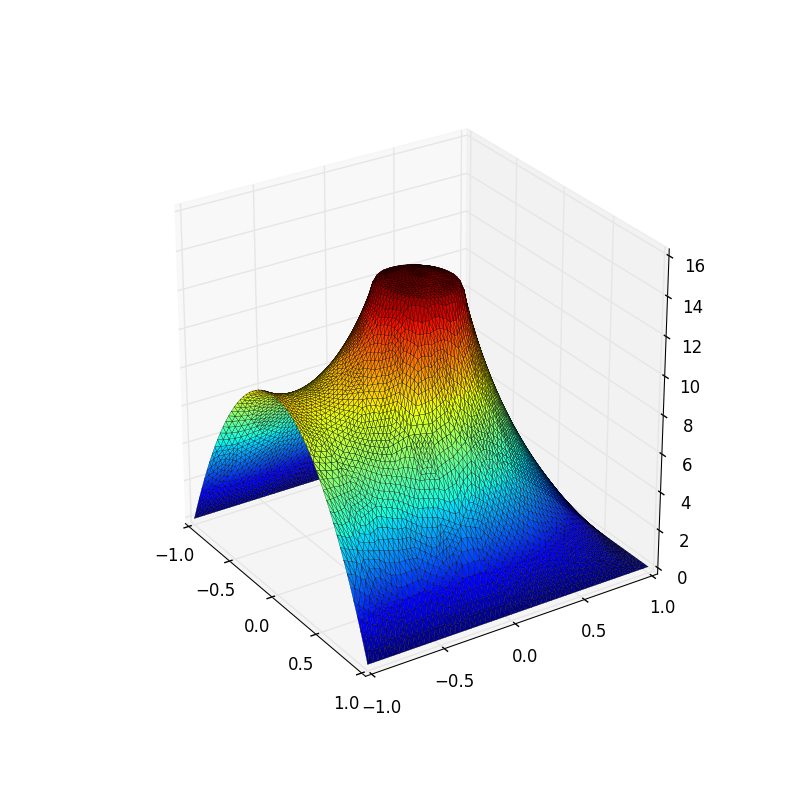
\includegraphics[width=0.8\textwidth]{given.PNG}
\caption{Computed solution for given $\kappa, f$ and boundary conditions. Quadratic elements, 2752 elements.}
\end{figure}

\section*{Is the accuracy improved?}
In order to determine the order of convergence an analytical test case was used to compare the computed solution with the exact solution:
\bes -\nabla \cdot \kappa \nabla u = -sin(x)\,sin(y), \; \kappa=1, \; u=0 \in d\Omega \ees
this permits the analytical solution:
\bes  u(x,y) = -\frac{1}{2 \pi^2}\,sin(x)\,sin(y) \ees

The discrete $l2$ norm of the error, $u - u^h$, was computed as:
\bes \sum_{\Omega} \int_\tau |J| \, (u^h-u)^2 d\mathbf{x} \approx \sum_{\Omega} |J| \sum_i \left( w_i u(\mathbf{x}_i) - u^h_i \right) \ees
where $u_i^h$ is the value of the computed solution at the interpolation points $x_i$ and $w_i$ the associated quadrature weights.

Figure 2 shows an example computed solution of this test case. Figure 3 plots the order of convergence of the two elements. It can be seen that not only is the accuracy of the quadratic elements better for the same number of elements, but the order of convergence is better as well. As expected the order of convergence of the linear elements was 1.00, while the quadratic element convergence rate was 1.86, almost in line with the expected value of 2.

\section*{How does the timing of the linear assembly scale? Does this change for quadratics?}
The assembly times for both linear and quadratic elements was measured for three refinement levels. Table 1 displays the timing in seconds. For both element types the assembly time was found to be proportional to the number of elements. Quadratic element assembly time was measured to take about 25\% longer than linear elements.
\begin{table}[!htb]
\centering
    \begin{tabular}{|l|l|l|l|}
        \hline
        Type/Num Elements & 688  & 2752 & 11008 \\ \hline
        Linear            & 0.14 secs & 0.57 & 2.20  \\
        Quadratic         & 0.18 & 0.70 & 2.77  \\
        \hline
    \end{tabular}
    \caption{Scaling of assembly time for $\mathbf{A}$ for linear and quadratic elements.}
\end{table}

\section*{Compare (an estimate of) the condition number. What can you conclude?}
Table 2 charts the scaling of the condition number given by \textit{numpy.linalg.cond(A.todense())}. It was found the condition number estimates given by \textit{scipy.sparse.linalg.lsmr()} were not accurate. Due to computational constraints the condition number couldn't be computed for the third refinement level.

Regardless, the scaling of the condition number is consistent; the condition number of quadratic elements is $\sim$ 5.8x that of linear elements, the condition number for both element types is proportional to $\sim$ 1.1x the number of elements. While quadratic elements converge more quickly then linear elements, the resulting linear system will likely require more iterations of a linear solver to reach the solution due to the higher condition number.
\begin{table}[!htb]
\centering
    \begin{tabular}{|l|l|l|l|}
        \hline
        Type/Num Elements & 688  & 2752 \\ \hline
        Linear            & 1452 & 6549  \\
        Quadratic         & 8533 & 38083 \\
        \hline
    \end{tabular}
    \caption{Scaling of condition number of $\mathbf{A}$ dependent on element type and number of elements.}
\end{table}

\newpage 
\begin{figure}[!htb]
\centering
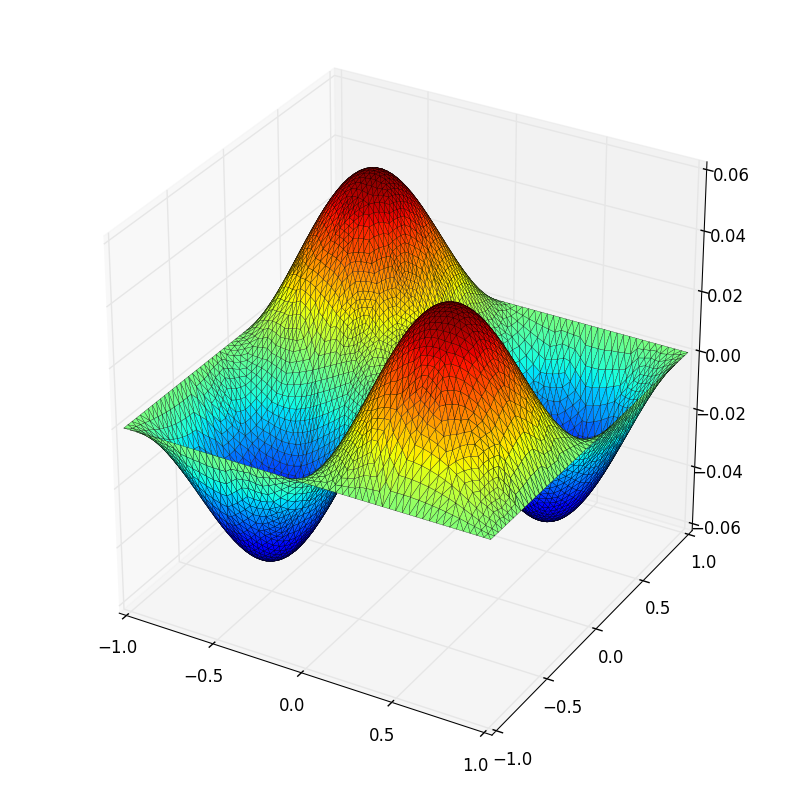
\includegraphics[width=0.7\textwidth]{periodic.PNG}
\caption{Example solution to the analytical test case, 2752 quadratic elements.}
\end{figure}

\begin{figure}[!htb]
\centering
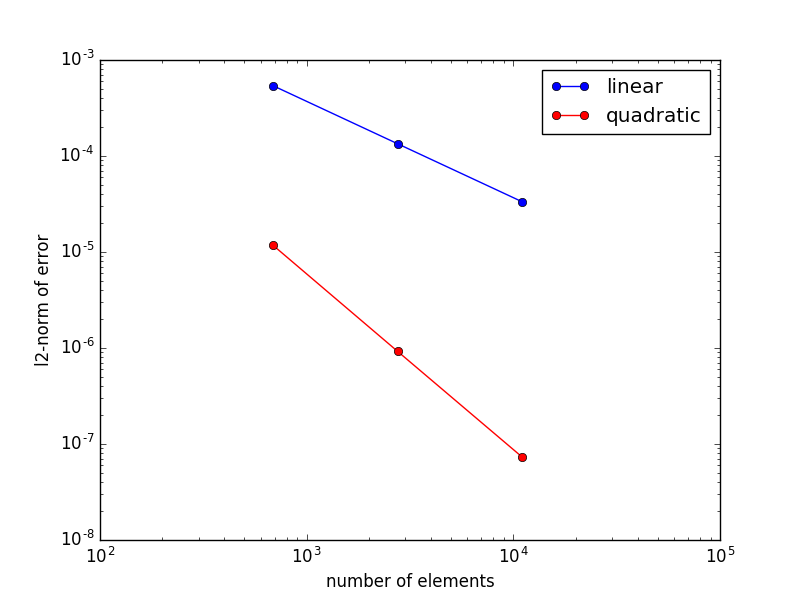
\includegraphics[width=0.8\textwidth]{convergence.PNG}
\caption{Convergence plots for linear and quadratic elements, 688,2752,11008 elements. Observed order of convergence for linear elements: 1.00, quadratic elements: 1.86}
\end{figure}

\section*{Compare the sparsity of the linear system for the linears versus quadratics.}
Figures 4 and 5 compare the sparsity of $\mathbf{A}$ for linear and quadratic elements. At first glance Figure 4 would indicate that the quadratic element is less sparse. However counting the number of non-zeros relative to matrix size, the linear element matrix is nearly 2.3x as dense.

The confusing figure can partially be blamed on the random numbering of the element vertices, particularly the triangle midpoints which were numbered without any care for optimality. If a Reverse Cuthill-Mckee ordering is computed to minimize the bandwidth a more understandable sparsity pattern emerges, as shown in Figure 5. It is evident from the plots that indeed the quadratic element matrix is more sparse, although it has nearly 4 times the bandwidth of the linear element matrix. The greater bandwidth shouldn't be surprising given the additional basis functions (and therefore the size of the element stencil) required for the quadratic element.
\begin{figure}[!htb]
\centering
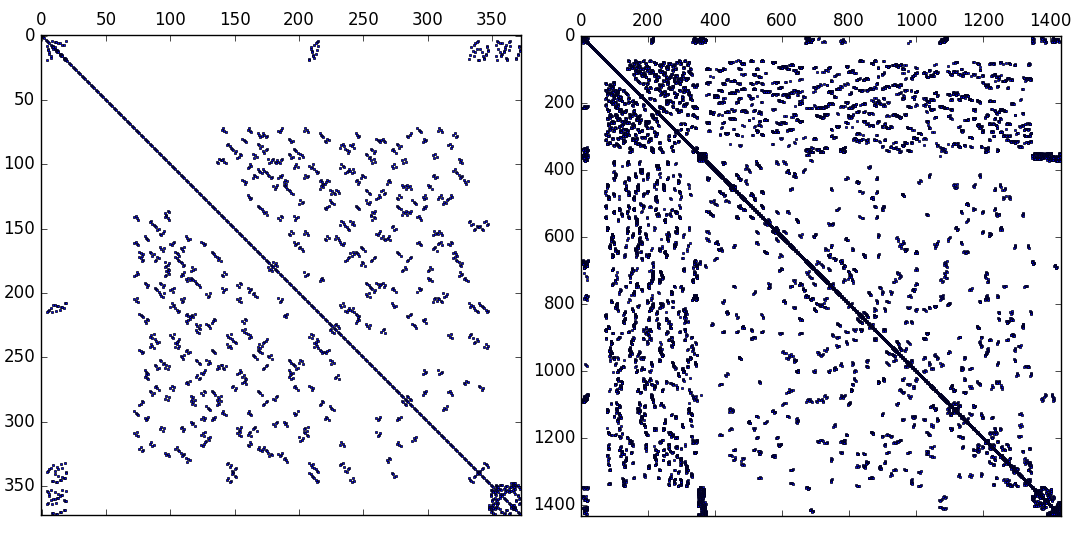
\includegraphics[width=1\textwidth]{spyLQ.PNG}
\caption{Sparsity pattern of $\mathbf{A}$ for linear(left) and quadratic(right) elements, 688 elements.}
\end{figure}

\begin{figure}[!htb]
\centering
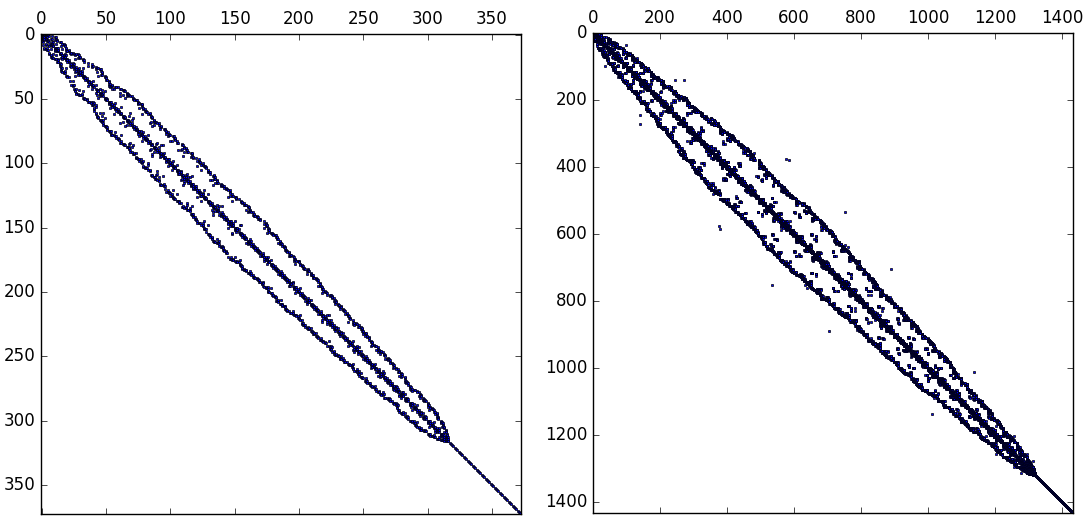
\includegraphics[width=1\textwidth]{spyLQ2.PNG}
\caption{Same matrices as in Figure 4, but after Reverse Cuthill-Mckee ordering.}
\end{figure}

\end{document}

%\begin{figure}[!htb]
%\centering
%\includegraphics[width=0.6\textwidth]{Unrolled.PNG}
%\caption{\label{fig:unrolled}"Unrolled" ring, coincident nodes at either end.}
%\end{figure}